\section{Optimization}

\subsection{Hybrid CORDAC}
\begin{frame}
    \frametitle{Hybrid CORDAC}
    	It retain the benefits of both iterative and recursive algorithms.
		Cache-efficient algorithm recursive subdivision continues until 
		the problem size becomes small enough.
	\begin{itemize}
		\item Asymptotic Improvement in Parallelism
		\item Highly Optimizable Base Cases
	\end{itemize}
\end{frame}

\subsection{Optimizing Kernel Functions}
\begin{frame}
    \frametitle{Optimizing Kernel Functions}
	Inside flexible kernel, 
	\begin{itemize}
		\item Copy-optimization: Copy the data into local $b \times b$ 
			static arrays.
		\item Loop Reordering: It is possible to change
			the looping order without hampering the correctness of the algorithms.
	\end{itemize}
\end{frame}

\subsection{Data Layout}
\begin{frame}
    \frametitle{Data Layout}
	\begin{figure}
		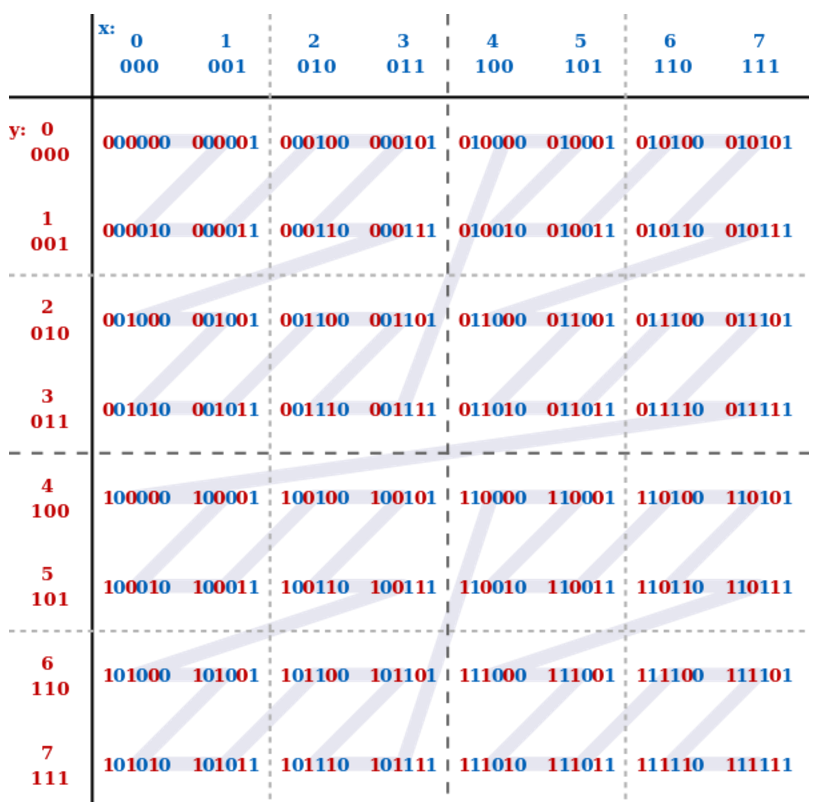
\includegraphics[scale=0.2]{figure/fig-z-morton.png}
	\end{figure}
	\begin{description}
		\item[Z-Morton Row-Major] ZM\_RM layout improves both temporal and 
			spatial localities.
	\end{description}
\end{frame}

\subsection{Auto vs. Explicit Vectorization}
\begin{frame}
    \frametitle{Auto vs. Explicit Vectorization}
	\begin{itemize}
		\item It often vectorize the base-case of the dominating kernel. 
		\item For example, $C_{\textit{loop}}$ is enough to get the 
			major share of the speedup.
	\end{itemize}
\end{frame}
